In the previous section we have seen the necessity to designed a device which do the polishing task in the fibers automatically. In this section we will explain it. This mechanical device, which we have designed, consists of two parts:

\begin{itemize}
\item On the one hand it have a metalic piece which hold and fix the papers that we use for polishing the fibers. We will move this piece instead of the piece which will hold the several fibers. The only reason of this decision is for mechanical simplicity.

Our objective is that we can describe the way which we want with this metalic piece in a bidimensional flat, whose size is delimited by the polishing papers and the position of the fibers which we are polishing. We have to take into account that, mathematicaly, we can describe any point inside of this flat with two non-parallel vectors so for moving inside of this flat we only need two screw, whose direction will be different. We will choose perpendicular directions for simplicity. You can see this configuration in the figure \ref{table}.

\begin{figure}[hbtp]
\centering
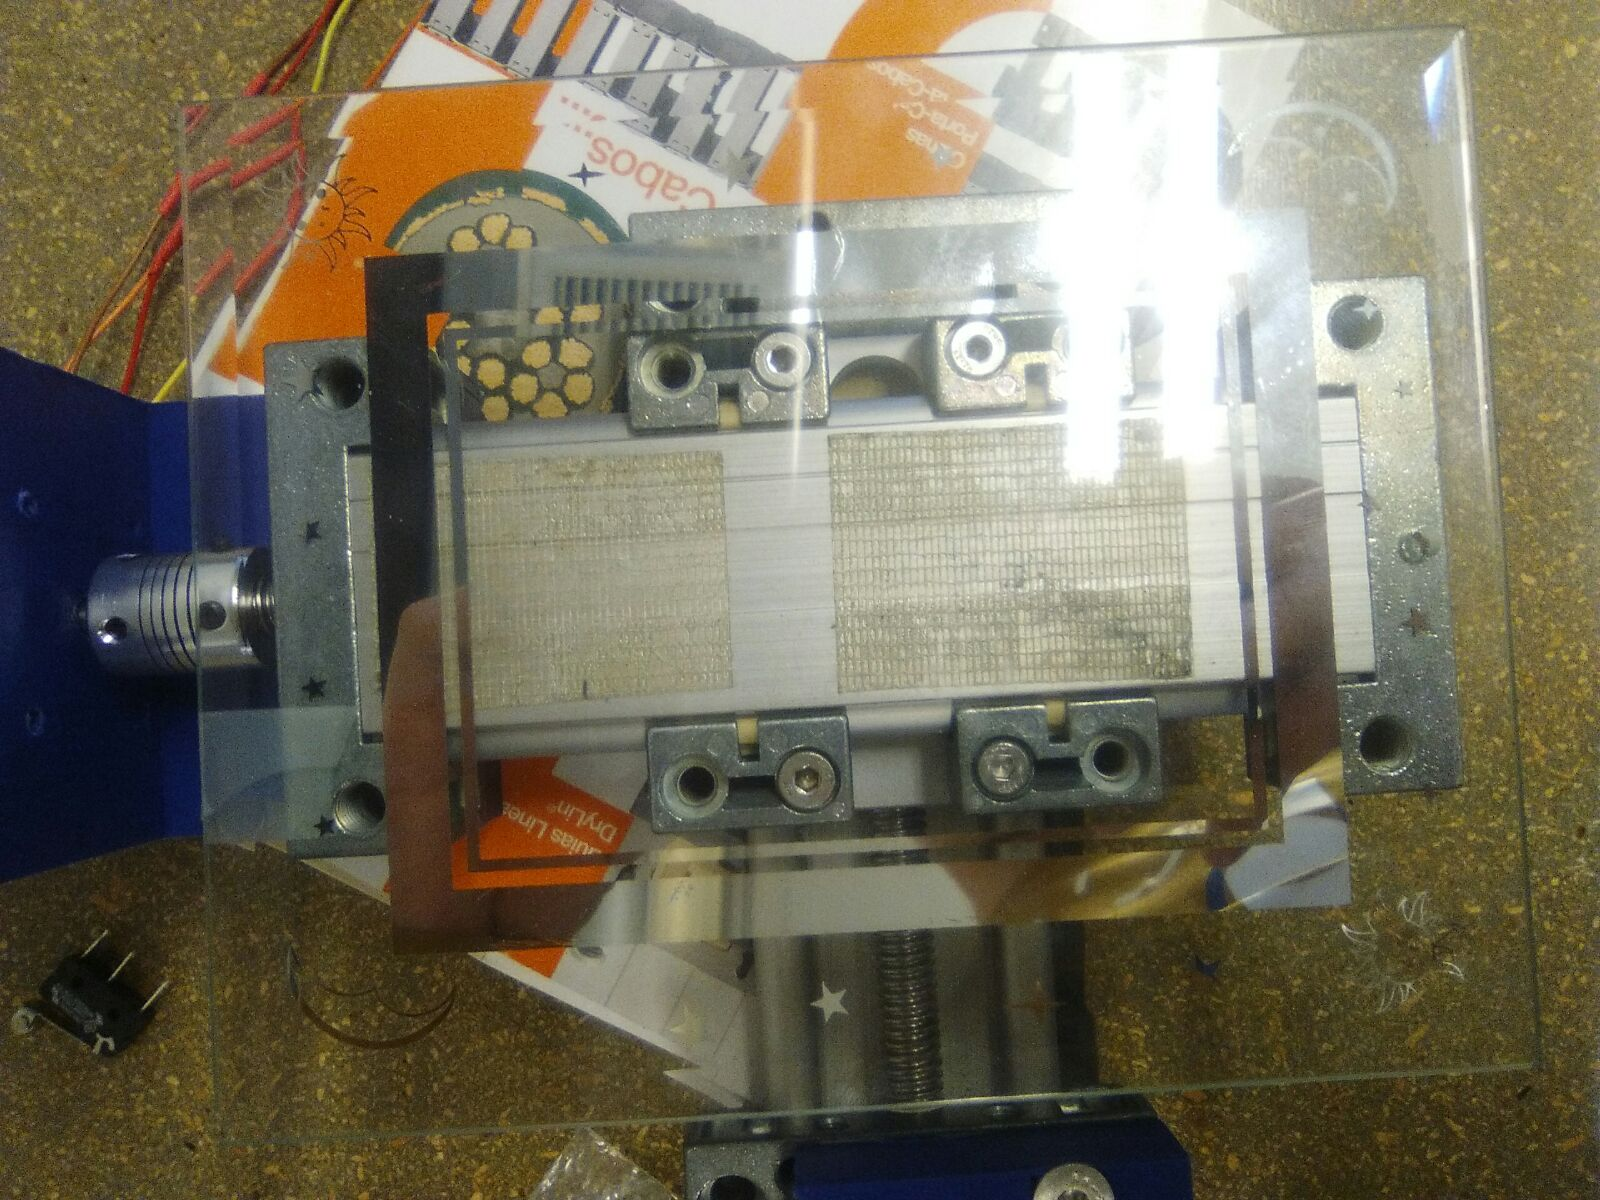
\includegraphics[scale=0.15]{../Figures/Table.jpeg}
\caption{Configuration of the table\label{table}}
\end{figure}

This device consist of two perpendiculas screws which are attached to a nut every one. The metalic piece, which hold the polishing papers, rest on both screws. When we move one nut out of both, the screw, which are attached, rotates. Therefore, the metalic piece move in this direction. As a result we can move this metalic piece following the way which we want inside of this flat with both nuts.

Hence we have a machine which is able to describe the movement which we want in a bidimensional flat with a pair of nuts. Now we only have to automate this movement. The idea is to connect a motor in every nut which we will control for doing this automatical movement. In the figure \ref{motors} you can observe both motors, every one of them are inside of every blue boxes and each one is connected to a nut. 

\begin{figure}[hbtp]
\centering
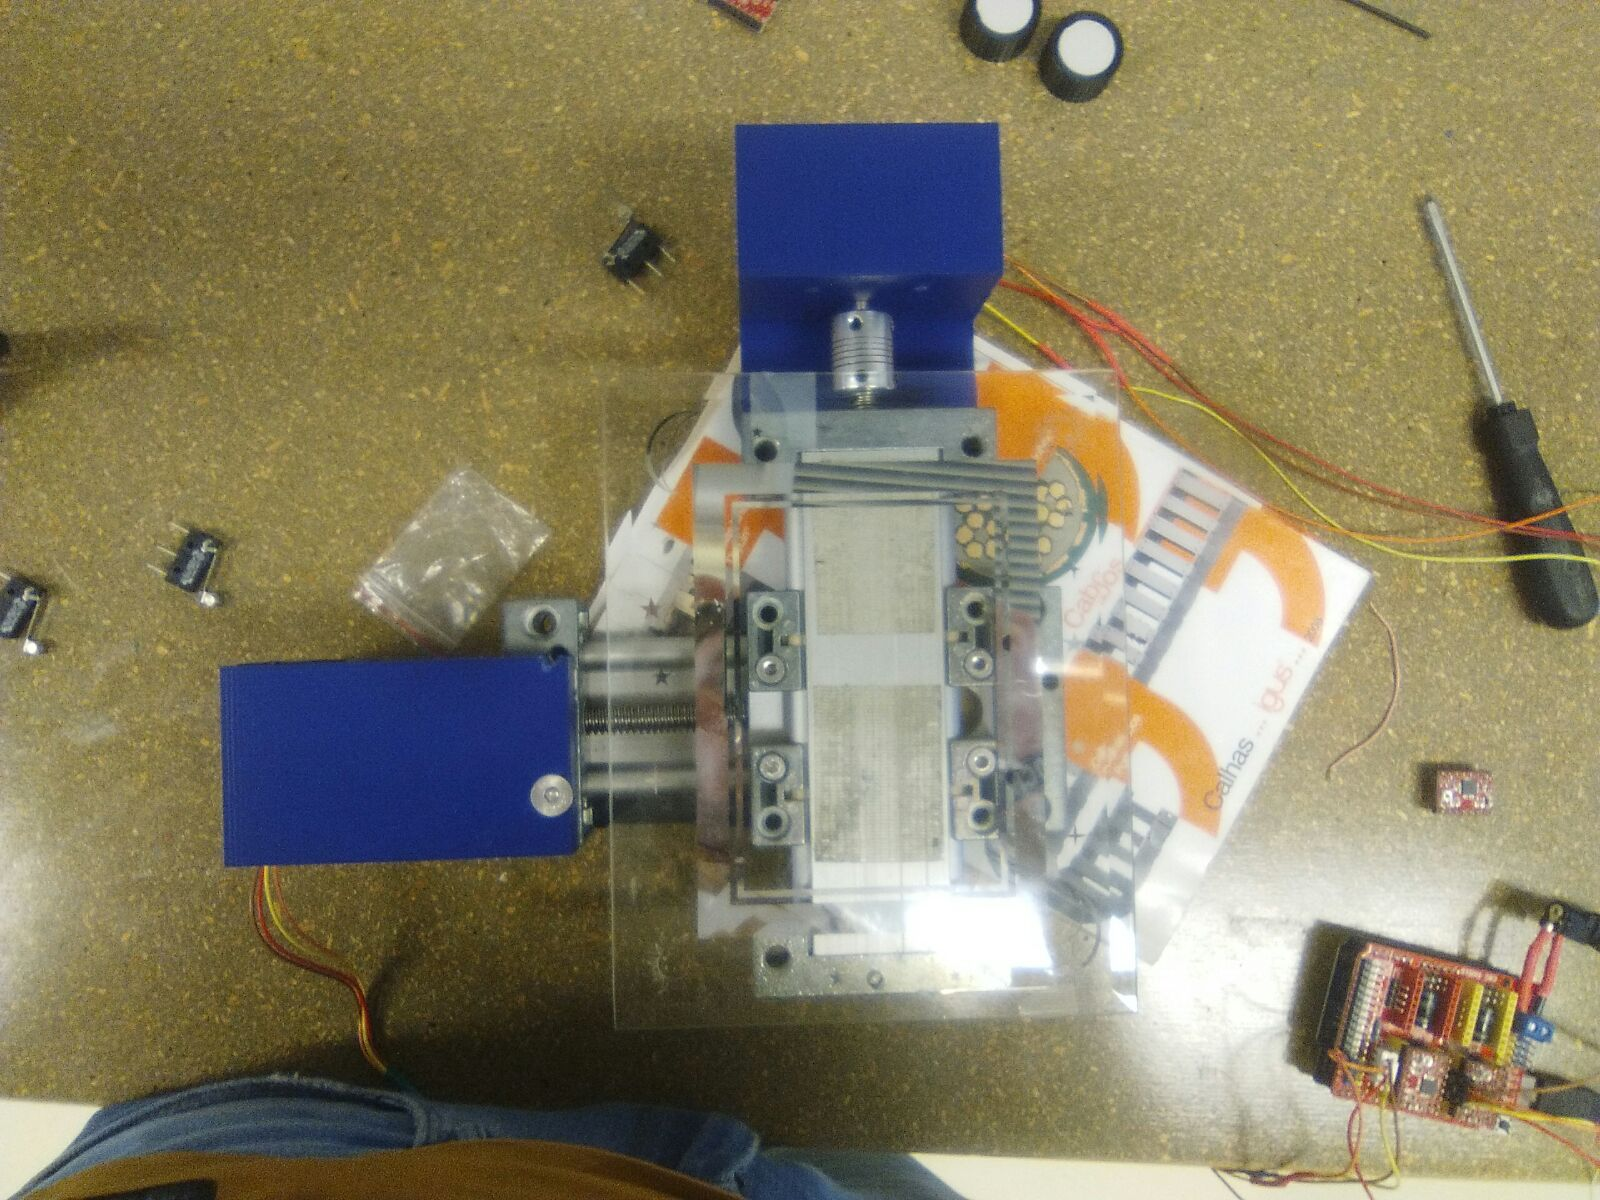
\includegraphics[scale=0.15]{../Figures/motors.jpeg}
\caption{Two motors connect to the nuts\label{motors}}
\end{figure}

So that we control both motors we are going to use arduino technology. Specifically we will use an arduino whose model is Genuino Uno Rev3 where we will connect a special card for working with motors. The name of this card is CNC SHIELD and I show it in the figure \ref{card}. You can observe that this card allow to connect 4 different microchips. Concrectly the microchip which we will use is 4988ET which is a DMOS Microstepping Driver with Translator and Overcurrent Protection and you can see it in the figure \ref{microchip}.

\begin{figure}[hbtp]
 \centering
  \subfloat[CNC SHIELD card\label{card}]{
    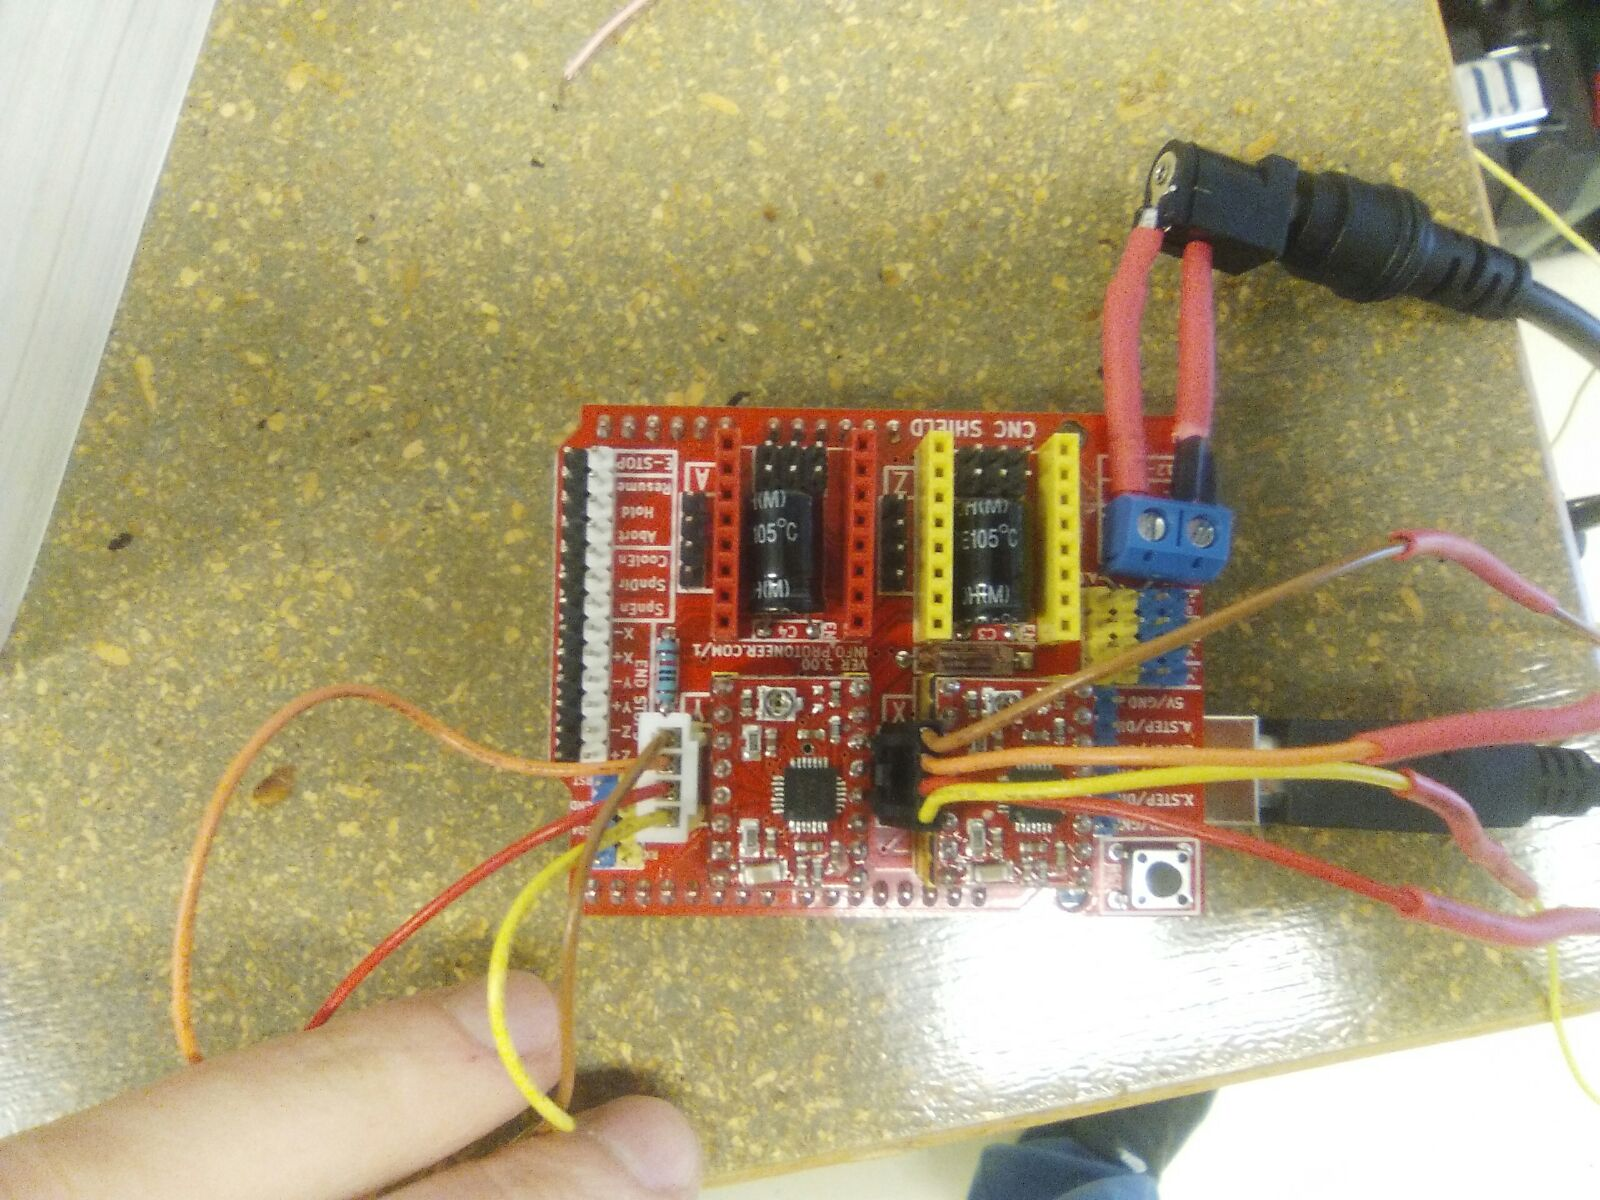
\includegraphics[width=0.5 \textwidth]{../Figures/card.jpeg}}
  \subfloat[4988ET\label{microchip}]{
    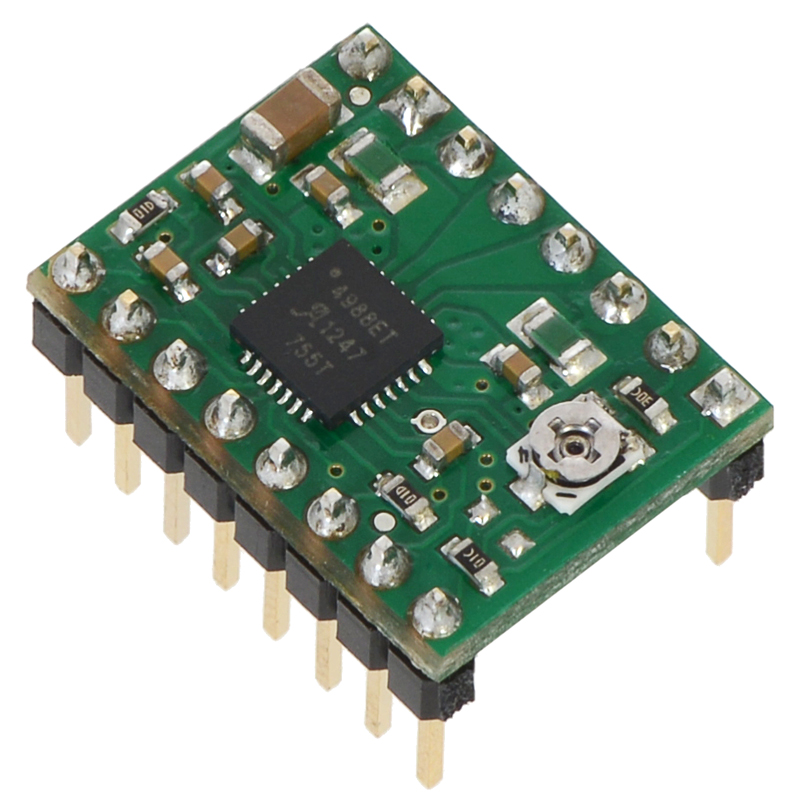
\includegraphics[width=0.5\textwidth]{../Figures/microchip.jpg}}
 \caption{Arduino technology. \label{technology}}
\end{figure}

As I said before this card allow to connect four different microchips and every microchip allow to control one different thing at the same time. As a result we can control 4 different things which could be 4 different motors if we want. By the moment we only need to control two motors for doing the movement which we want so we can reserve this other connections for doing other things. The main idea is to use one out of two rest connections for programing a emergency stop. For instance we can do it if we can use a switch, like the switch which appear in the figure \ref{switch}. We can put a switch in every limit of metalic piece way, which we move, along the every screw (in both sides). In this case, if this metalic piece arrive to this limit along the screws, it will press this switch and this movimint will stop fastly. In this way we can avoid misused of this machine that could affect to the operation of this device. The electronical circuit, which control this switch, could be really simply. We only need a typical electronic circuit, which is normal open but, when the metalic piece press the switch, this circuit will close. In this case we will have a signal that will travel in this circuit and will arrive to the arduino which, when received this signal, will stop.


\begin{figure}[hbtp]
\centering
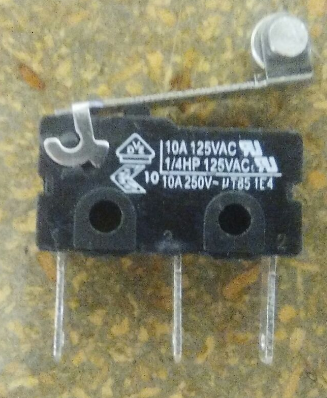
\includegraphics[scale=0.5]{../Figures/switch.png}
\caption{Switch for emergency stop\label{switch}}
\end{figure}

\item On the other hand it have one piece which hold several fibers. This piece is really simply. We only need that this piece can hold several fibers at the same time. For simplicity this piece will be fix when we are polishing and, as I said before, we will move the metalic piece.

Moreover we have to take into account that it is really important that both flat (the piece which hold the fibers and the metalic piece) to be parallel so that we can get the spatial accuracy which we want. You can see the piece, which we have designed for holding the fibers, in the figure \ref{hold25fibers}

\begin{figure}[hbtp]
\centering
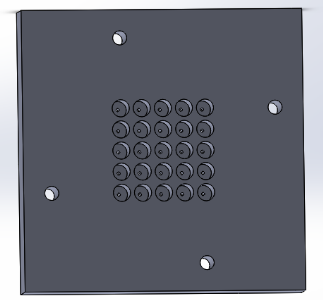
\includegraphics[scale=0.5]{../Figures/metalicpiece.png}
\caption{Piece which hold the fibers\label{hold25fibers}}
\end{figure}


We have designed this piece with one hold in every side where we will put a screw in every one for holding this piece and connecting both piece. Therefore we can change the orientation of this piece respect to the metalic piece with this screws for getting that both flats are parallel.

Moreover we have several holes for holding the fibers. In concret these holes have two diameters as you can see in the figure \ref{hold25fibers}. We have first a bigger diameter where we pass the fiber and a metalic piece which we need for increase the weight of every fiber. With this bigger diameter we get to fix the fiber and this metalic piece for safety reasons. You can see this metalic piece in the figure \ref{metalicpiece}. 

\begin{figure}[hbtp]
\centering
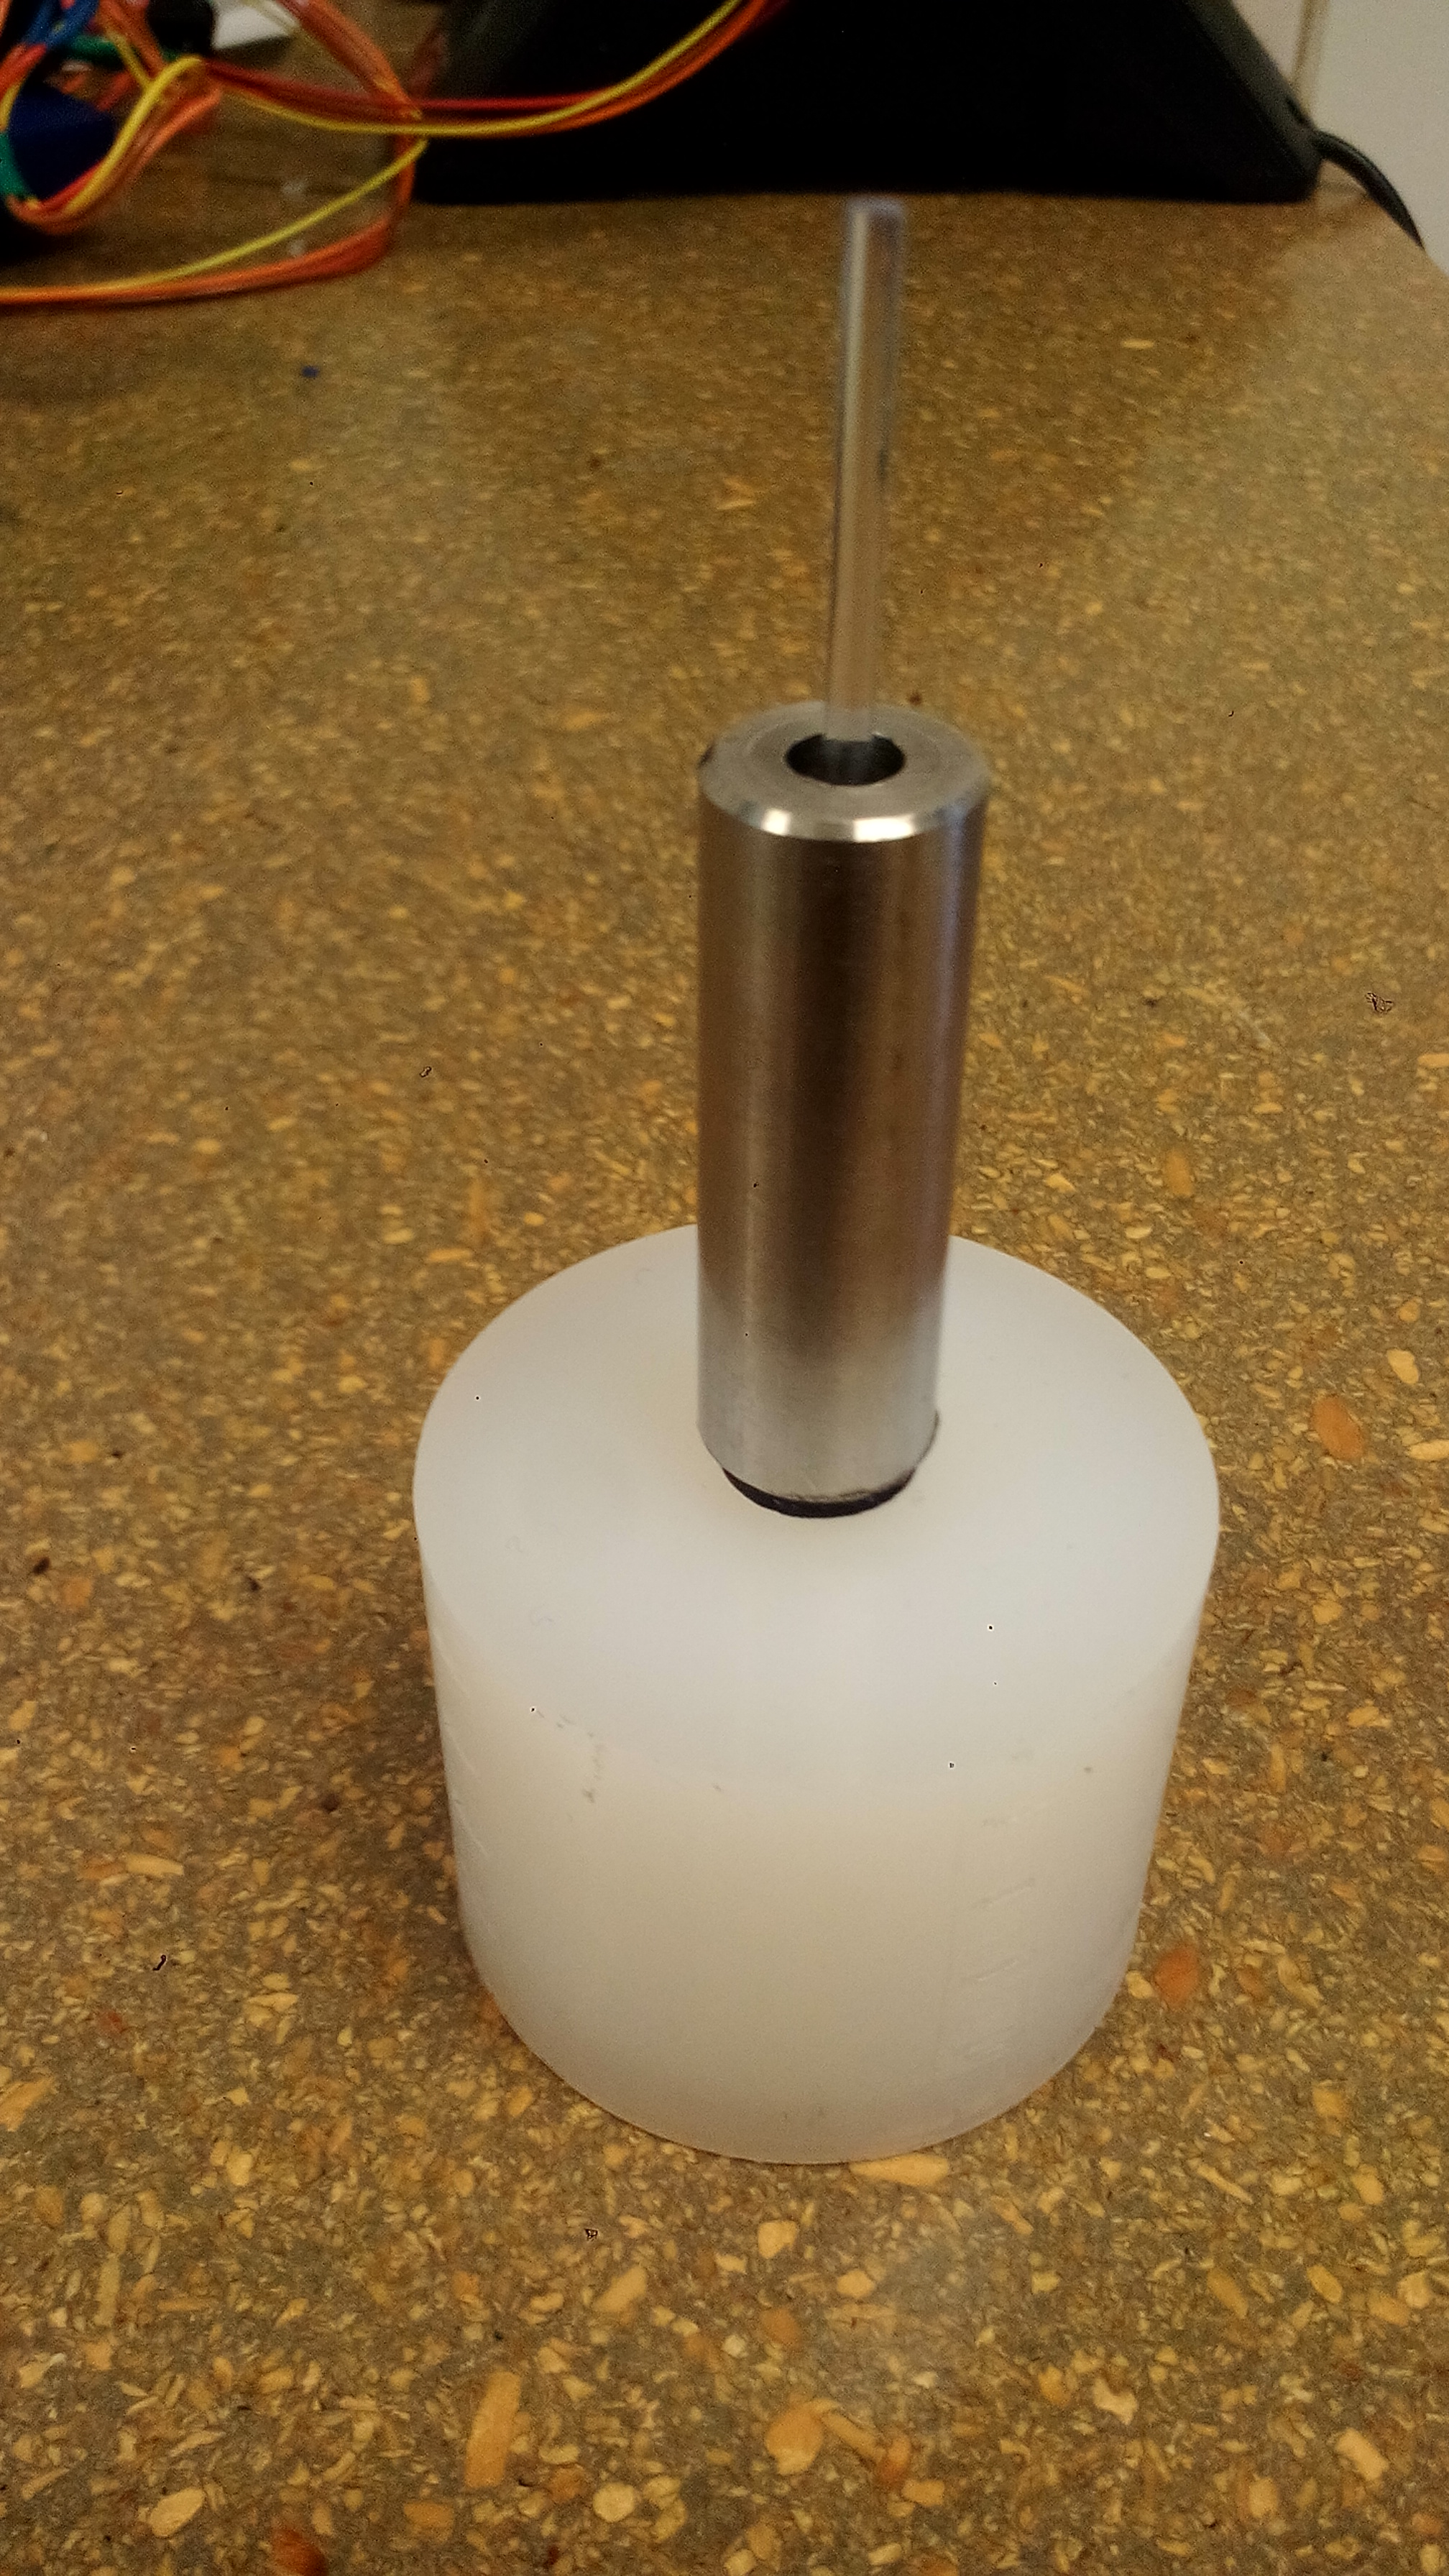
\includegraphics[scale=0.05]{../Figures/piece.jpg}
\caption{Metalic piece which press every fiber\label{metalicpiece}}
\end{figure}

The weight of this piece is more or less $100~\gram$. We have checked that with this weight we can obtain a good results when we polish but we want to check what is the minimum weight of this piece with which we obtain the best results because the smaller weight of this piece, the lower damage we obtain in the fiber. We will fix this metalic piece to every fiber with a plastic belt whose position will mark the maximum distance which we loss when we polish this fiber. 

Finally, every hole of the piece, which hold the fibers, will have another smallest diameter where we only pass the fiber.

As this piece isn't in contact to the piece which is moving when we are polishing we can use the material which we want for designing this piece since this won't affect to the result. We can use a cheaper material which have little weight. The piece which you can see in the figura \ref{hold25fibers} only have twenty five holes so you only can hold twenty five fibers at the same time. It isn't important because this piece is cheaper so you can designed other similar piece which have very many holes if your experiment need it. 
\end{itemize}

Until now we have described this device. Now we are going to speak about the code which we will use for automate this device. 

We have several options for doing this programmating task. By he moment we are going to program directly the CNC SHIELD (special card) instead of programing the arduino. The problem is that we have to learn other different programing language, whose name is Gcode but with this we obtain a big profit because Gcode is a pseudocode and, as I said before, this card is specially prepare for working with motors so there are a lot of functions which will be really useful for our task. As a result we will need less code with this programming language for doing the same task.     

By the moment we are working in line from the computer for controling this motors but our final idea is to write a gcode in a python file and upload this file in the arduino. In this case, We won't need a laptop for controling this device. Moreover if we use a battery we will have a portable devices.